% !TEX root = ../Documentation.tex

\subsection{System overview}
\label{design:system-overview}
  The parser module overview is given in \autoref{fig:ParserModules}.
  \begin{figure}[ht]%
    \centering
    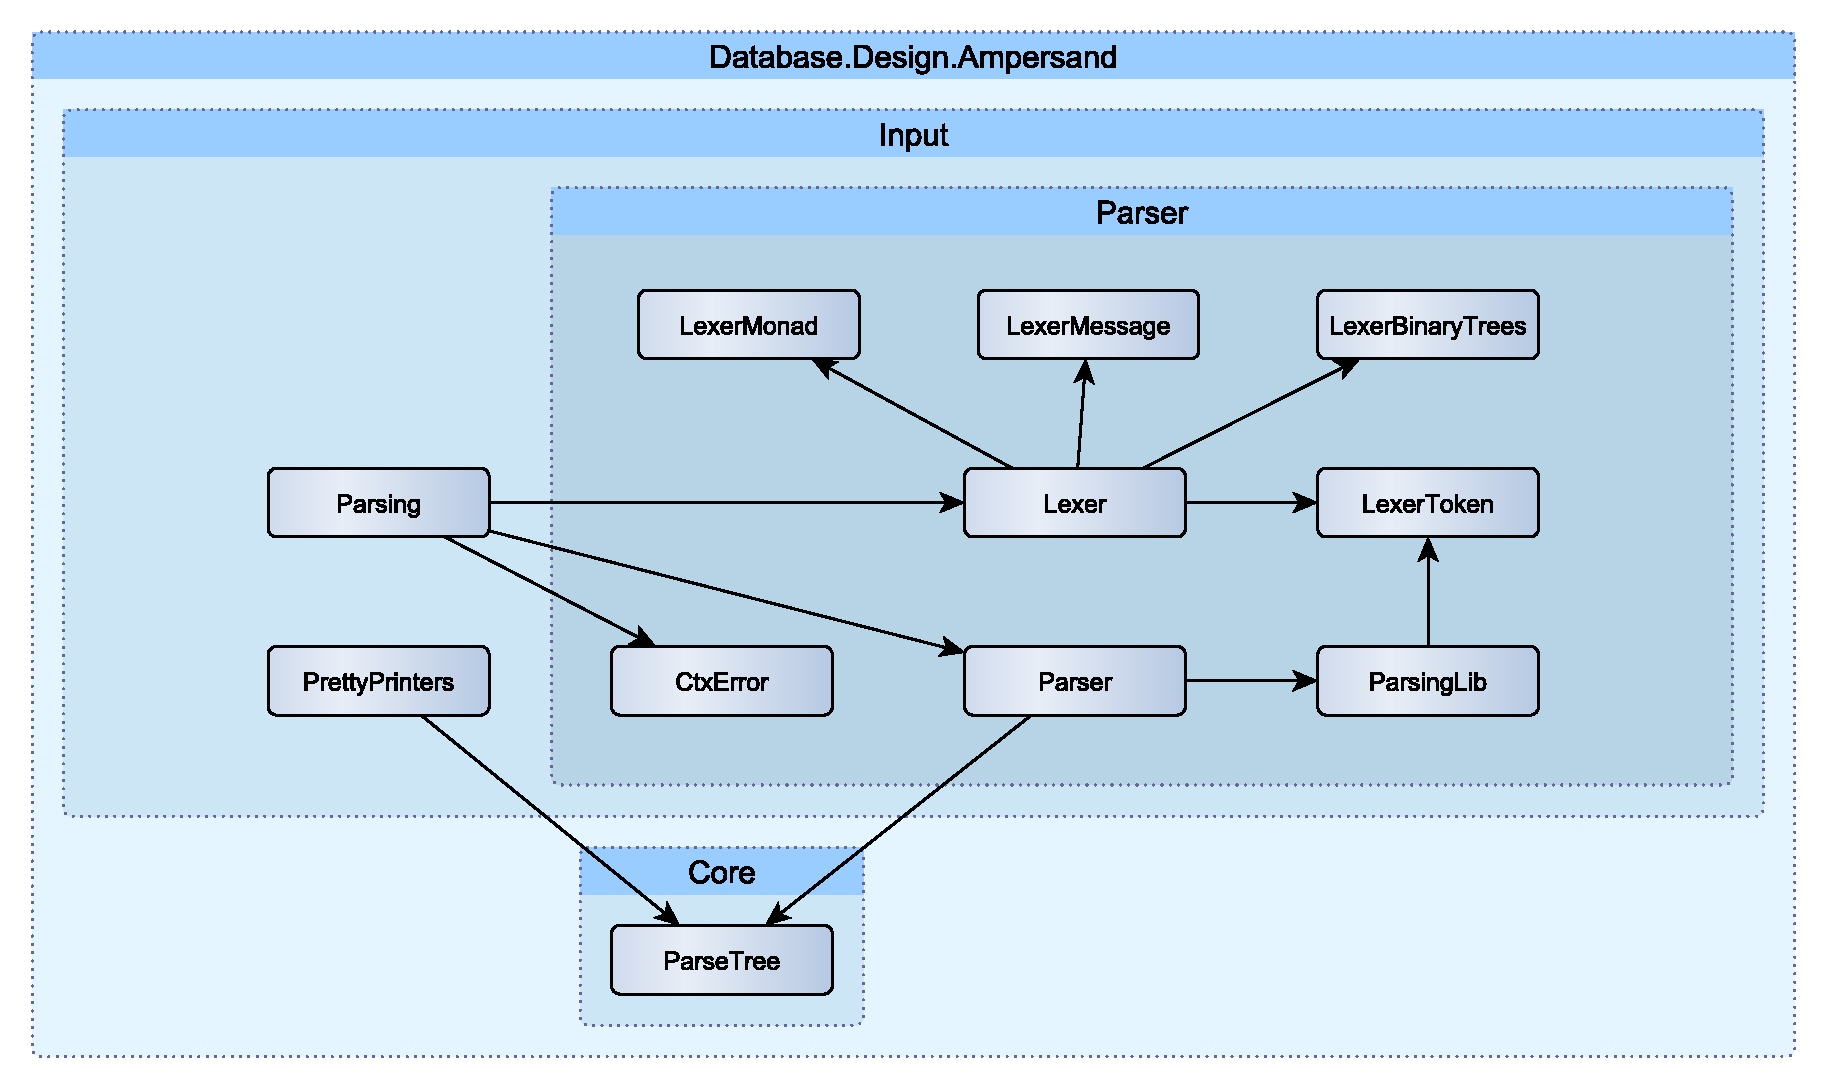
\includegraphics[width=0.7\columnwidth]{Figures/ParserModules}
    \caption{The modules relevant for the parser and their relationships}
    \label{fig:ParserModules}
  \end{figure}%
  Each module has the following responsibilities:
  %
  \begin{description}
    \item[Parsing] module that implements the interface of the parser with the rest of the system.
      It is responsible for reading the input files, calling the lexer and the parser and returning a parse tree as result (or a parse error).

    \item[Parser] module responsible for executing the parsing itself.
      It accepts the tokens that are allowed in each grammar production and generates the corresponding parse tree.
      The parser is described in \autoref{design:new-parser}.
      
    \item[ParsingLib] library that contains several useful functions to assist the parser, e.g. token recognition.
      These functions are not depending on the specific grammar rules.
      
    \item[ParseTree] external module containing the parse tree data structures.
      Only details of this module have been changed during this project (e.g. field ordering).
    
    \item[PrettyPrinters] contains the \code{Pretty} class and the functions responsible for printing the parse tree to ADL scripts in a `pretty' way.
    
    \item[CtxError] contains the data structures responsible for the parse errors and their location.
      This module has not been refactored as a part of this project.
    
    \item[Lexer/LexerToken] modules responsible for recognizing the input characters and converting them to tokens.
      The new lexer, together with its sub-modules, is described in \autoref{design:new-lexer}.
  \end{description}
